%%%%%%%%%%%%%%%%%%%%%%%%%%%%%%%%%%%%%%%%%
% Programming/Coding Assignment
% LaTeX Template
%
% This template has been downloaded from:
% http://www.latextemplates.com
%
% Original author:
% Ted Pavlic (http://www.tedpavlic.com)
%
% Note:
% The \lipsum[#] commands throughout this template generate dummy text
% to fill the template out. These commands should all be removed when 
% writing assignment content.
%
% This template uses a Perl script as an example snippet of code, most other
% languages are also usable. Configure them in the "CODE INCLUSION 
% CONFIGURATION" section.
%
%%%%%%%%%%%%%%%%%%%%%%%%%%%%%%%%%%%%%%%%%

%----------------------------------------------------------------------------------------
%	PACKAGES AND OTHER DOCUMENT CONFIGURATIONS
%----------------------------------------------------------------------------------------

\documentclass{article}

\usepackage{fancyhdr} % Required for custom headers
\usepackage{lastpage} % Required to determine the last page for the footer
\usepackage{extramarks} % Required for headers and footers
\usepackage[usenames,dvipsnames]{color} % Required for custom colors
\usepackage{graphicx} % Required to insert images
\usepackage{listings} % Required for insertion of code
\usepackage{courier} % Required for the courier font
\usepackage{lipsum} % Used for inserting dummy 'Lorem ipsum' text into the template
\usepackage{setspace}
\usepackage{color}
\usepackage{comment}
\usepackage{caption}

\usepackage{hyperref}
\usepackage{natbib}
\usepackage{underscore}
\usepackage{subfigure}


\hypersetup{
    colorlinks=true,
    linkcolor=blue,
    filecolor=magenta,      
    urlcolor=cyan,
    breaklinks=true
}

%\usepackage[]{algorithm2e}
\usepackage{pdfpages}




%For python inclusion (http://widerin.org/blog/syntax-highlighting-for-python-scripts-in-latex-documents)
\definecolor{Code}{rgb}{0,0,0}
\definecolor{Decorators}{rgb}{0.5,0.5,0.5}
\definecolor{Numbers}{rgb}{0.5,0,0}
\definecolor{MatchingBrackets}{rgb}{0.25,0.5,0.5}
\definecolor{Keywords}{rgb}{0,0,1}
\definecolor{self}{rgb}{0,0,0}
\definecolor{Strings}{rgb}{0,0.63,0}
\definecolor{Comments}{rgb}{0,0.63,1}
\definecolor{Backquotes}{rgb}{0,0,0}
\definecolor{Classname}{rgb}{0,0,0}
\definecolor{FunctionName}{rgb}{0,0,0}
\definecolor{Operators}{rgb}{0,0,0}
\definecolor{Background}{rgb}{0.98,0.98,0.98}

% Margins
\topmargin=-0.45in
\evensidemargin=0in
\oddsidemargin=0in
\textwidth=6.5in
\textheight=9.0in
\headsep=0.25in

\linespread{1.1} % Line spacing

% Set up the header and footer
\pagestyle{fancy}
\lhead{\hmwkAuthorName} % Top left header
%\chead{\hmwkClass\ (\hmwkClassInstructor\ \hmwkClassTime): \hmwkTitle} % Top center head
\chead{\hmwkClass\ (\hmwkClassInstructor): \hmwkTitle} % Top center head
\rhead{\firstxmark} % Top right header
\lfoot{\lastxmark} % Bottom left footer
\cfoot{} % Bottom center footer
\rfoot{Page\ \thepage\ of\ \protect\pageref{LastPage}} % Bottom right footer
\renewcommand\headrulewidth{0.4pt} % Size of the header rule
\renewcommand\footrulewidth{0.4pt} % Size of the footer rule

\setlength\parindent{0pt} % Removes all indentation from paragraphs

%----------------------------------------------------------------------------------------
%	CODE INCLUSION CONFIGURATION
%----------------------------------------------------------------------------------------

\definecolor{MyDarkGreen}{rgb}{0.0,0.4,0.0} % This is the color used for comments
\lstloadlanguages{Perl} % Load Perl syntax for listings, for a list of other languages supported see: ftp://ftp.tex.ac.uk/tex-archive/macros/latex/contrib/listings/listings.pdf
\lstset{language=Perl, % Use Perl in this example
        frame=single, % Single frame around code
        basicstyle=\small\ttfamily, % Use small true type font
        keywordstyle=[1]\color{Blue}\bf, % Perl functions bold and blue
        keywordstyle=[2]\color{Purple}, % Perl function arguments purple
        keywordstyle=[3]\color{Blue}\underbar, % Custom functions underlined and blue
        identifierstyle=, % Nothing special about identifiers                                         
        commentstyle=\usefont{T1}{pcr}{m}{sl}\color{MyDarkGreen}\small, % Comments small dark green courier font
        stringstyle=\color{Purple}, % Strings are purple
        showstringspaces=false, % Don't put marks in string spaces
        tabsize=5, % 5 spaces per tab
        %
        % Put standard Perl functions not included in the default language here
        morekeywords={rand},
        %
        % Put Perl function parameters here
        morekeywords=[2]{on, off, interp},
        %
        % Put user defined functions here
        morekeywords=[3]{test},
       	%
        morecomment=[l][\color{Blue}]{...}, % Line continuation (...) like blue comment
        numbers=left, % Line numbers on left
        firstnumber=1, % Line numbers start with line 1
        numberstyle=\tiny\color{Blue}, % Line numbers are blue and small
        stepnumber=5 % Line numbers go in steps of 5
}

% Creates a new command to include a perl script, the first parameter is the filename of the script (without .pl), the second parameter is the caption
\newcommand{\perlscript}[2]{
\begin{itemize}
\item[]\lstinputlisting[caption=#2,label=#1]{#1.pl}
\end{itemize}
}


%----------------------------------------------------------------------------------------
%	DOCUMENT STRUCTURE COMMANDS
%	Skip this unless you know what you're doing
%----------------------------------------------------------------------------------------

% Header and footer for when a page split occurs within a problem environment
\newcommand{\enterProblemHeader}[1]{
\nobreak\extramarks{#1}{#1 continued on next page\ldots}\nobreak
\nobreak\extramarks{#1 (continued)}{#1 continued on next page\ldots}\nobreak
}

% Header and footer for when a page split occurs between problem environments
\newcommand{\exitProblemHeader}[1]{
\nobreak\extramarks{#1 (continued)}{#1 continued on next page\ldots}\nobreak
\nobreak\extramarks{#1}{}\nobreak
}

\setcounter{secnumdepth}{0} % Removes default section numbers
\newcounter{homeworkProblemCounter} % Creates a counter to keep track of the number of problems

\newcommand{\homeworkProblemName}{}
\newenvironment{homeworkProblem}[1][Problem \arabic{homeworkProblemCounter}]{ % Makes a new environment called homeworkProblem which takes 1 argument (custom name) but the default is "Problem #"
\stepcounter{homeworkProblemCounter} % Increase counter for number of problems
\renewcommand{\homeworkProblemName}{#1} % Assign \homeworkProblemName the name of the problem
\section{\homeworkProblemName} % Make a section in the document with the custom problem count
\enterProblemHeader{\homeworkProblemName} % Header and footer within the environment
}{
\exitProblemHeader{\homeworkProblemName} % Header and footer after the environment
}

\newcommand{\problemAnswer}[1]{ % Defines the problem answer command with the content as the only argument
\noindent\framebox[\columnwidth][c]{\begin{minipage}{0.98\columnwidth}#1\end{minipage}} % Makes the box around the problem answer and puts the content inside
}

\newcommand{\homeworkSectionName}{}
\newenvironment{homeworkSection}[1]{ % New environment for sections within homework problems, takes 1 argument - the name of the section
\renewcommand{\homeworkSectionName}{#1} % Assign \homeworkSectionName to the name of the section from the environment argument
\subsection{\homeworkSectionName} % Make a subsection with the custom name of the subsection
\enterProblemHeader{\homeworkProblemName\ [\homeworkSectionName]} % Header and footer within the environment
}{
\enterProblemHeader{\homeworkProblemName} % Header and footer after the environment
}

%----------------------------------------------------------------------------------------
%	NAME AND CLASS SECTION
%----------------------------------------------------------------------------------------

\newcommand{\hmwkTitle}{Assignment\ \#9 } % Assignment title
%\newcommand{\hmwkDueDate}{Monday,\ January\ 1,\ 2012} % Due date
\newcommand{\hmwkClass}{Introduction to Web Science} % Course/class
%\newcommand{\hmwkClassTime}{10:30am} % Class/lecture time
\newcommand{\hmwkClassInstructor}{Dr. Nelson} % Teacher/lecturer
\newcommand{\hmwkAuthorName}{Alexander Nwala} % Your name

%----------------------------------------------------------------------------------------
%	TITLE PAGE
%----------------------------------------------------------------------------------------

\title{
\vspace{2in}
\textmd{\textbf{\hmwkClass:\ \hmwkTitle}}\\
%\normalsize\vspace{0.1in}\small{Due\ on\ \hmwkDueDate}\\
%\vspace{0.1in}\large{\textit{\hmwkClassInstructor\ \hmwkClassTime}}
\vspace{0.1in}\large{\textit{\hmwkClassInstructor}}
\vspace{3in}
}

\author{\textbf{\hmwkAuthorName}}
\date{Thursday, December 4, 2014} % Insert date here if you want it to appear below your name

%----------------------------------------------------------------------------------------

\begin{document}

\maketitle



%----------------------------------------------------------------------------------------
%	TABLE OF CONTENTS
%----------------------------------------------------------------------------------------

%\setcounter{tocdepth}{1} % Uncomment this line if you don't want subsections listed in the ToC

\newpage
\tableofcontents
\newpage

%----------------------------------------------------------------------------------------
%	PROBLEM 1
%----------------------------------------------------------------------------------------

% To have just one problem per page, simply put a \clearpage after each problem

\begin{homeworkProblem}

(10 points; 2 points for each question and 2 points for aesthetics)\\

Support your answer: include all relevant discussion, assumptions,
examples, etc.\\

Create a blog-term matrix.  Start by grabbing 100 blogs; include:\\

\url{http://f-measure.blogspot.com/}\\
\url{http://ws-dl.blogspot.com/}\\

and grab 98 more as per the method shown in class.\\

Use the blog title as the identifier for each blog (and row of the
matrix).  Use the terms from every item/title (RSS) or entry/title
(Atom) for the columns of the matrix.  The values are the frequency
of occurrence.  Essentially you are replicating the format of the
``blogdata.txt'' file included with the PCI book code.  Limit the
number of terms to the most ``popular'' (i.e., frequent) 500 terms,
this is *after* the criteria on p. 32 (slide 7) has been satisfied.\\

Create a histogram of how many pages each blog has (e.g., 30
blogs with just one page, 27 with two pages, 29 with 3 pages and 
so on).  

%\problemAnswer
%{
    \begin{verbatim}\end{verbatim}
    \textbf{SOLUTION 1}\\

    The solution for this problem is outlined by the following steps:
    \begin{enumerate}

    \item \textbf{Collect 98 blogs:} This was achieved by continuously retrieving the url due to invoking the head of \url{http://www.blogger.com/next-blog?navBar=true&blogID=3471633091411211117}, as outlined by Listing 1.

    \lstinputlisting[breaklines=true, caption=Grab 100 Unique Blogs]{grabUniqueBlogsSnippet.py}

    \item \textbf{Generate blog matrix:} This was achieved by utilizing the PCI book's \cite{pciBook} generatefeedvector.py with the additional modification of exploring multiple pages (pagination) of blogs as outlined in Listing 2.

    \begin{verbatim}
        The file blogVector.txt contains the blog matrix
    \end{verbatim}

    \lstinputlisting[breaklines=true, caption=Generate Blog Matrix]{genBlogMatrixSnippet.py}

    
    \item \textbf{Limit the number of terms to the 500 most ``popular'':} This was achieved my adding the following block (Listing 3.) into generatefeedvector.py

    \lstinputlisting[breaklines=true, caption=500 Most Popular Blogs]{mostPopularBlogsSnippet.py}

    \item \textbf{Create blog page count histogram:} This was achieved due to Listing 4. (Generated the data) and Listing 5. (Plotted the data - Figure 1). Pagination was achieved due to the recursive method recursivelyGetFeedPagesForBlog() (Listing 4.) which continued to get the links to the next page until no link was available.

    \lstinputlisting[breaklines=true, caption=Generate Blog Histogram]{genBlogPageCountHistogramSnippet.py}
    \lstinputlisting[breaklines=true, caption=Plot Blog Histogram]{../blogPageCountHist.r}

    \end{enumerate}
    
    \begin{figure}
        \caption{Distribution of Pages}
        \subfigure{\includegraphics[width=\textwidth]{../Rplots.pdf}}
    \end{figure}

%}



\end{homeworkProblem}

%----------------------------------------------------------------------------------------
%	PROBLEM 2
%----------------------------------------------------------------------------------------
\begin{homeworkProblem}

Create an ASCII and JPEG dendrogram that clusters (i.e., HAC)
the most similar blogs (see slides 12 \& 13).  Include the JPEG in
your report and upload the ascii file to github (it will be too
unwieldy for inclusion in the report).

\begin{verbatim}\end{verbatim}
\textbf{SOLUTION 2}\\


The solution for this problem is outlined by the following steps:
\begin{enumerate}

\item \textbf{Create dendograms:} This was achieved due to Listing 6. Figure 2. shows the JPEG dendogram and Listing 7. contains an excerpt of the ASCII dendogram.

\begin{verbatim}
    The file blogAsciiDendogram.txt contains the ASCII blog dendogram
    The file blogclust.jpg contains the Jpeg blog dendogram
\end{verbatim}

\lstinputlisting[breaklines=true, caption=Create Dendograms]{createDendogramsSnippet.py}
\lstinputlisting[breaklines=true, caption=Blogs ASCII Dendogram Excerpt]{../blogAsciiDendogramSnippet.txt}

\begin{figure}
    \caption{Blogs Dendogram}
    \subfigure{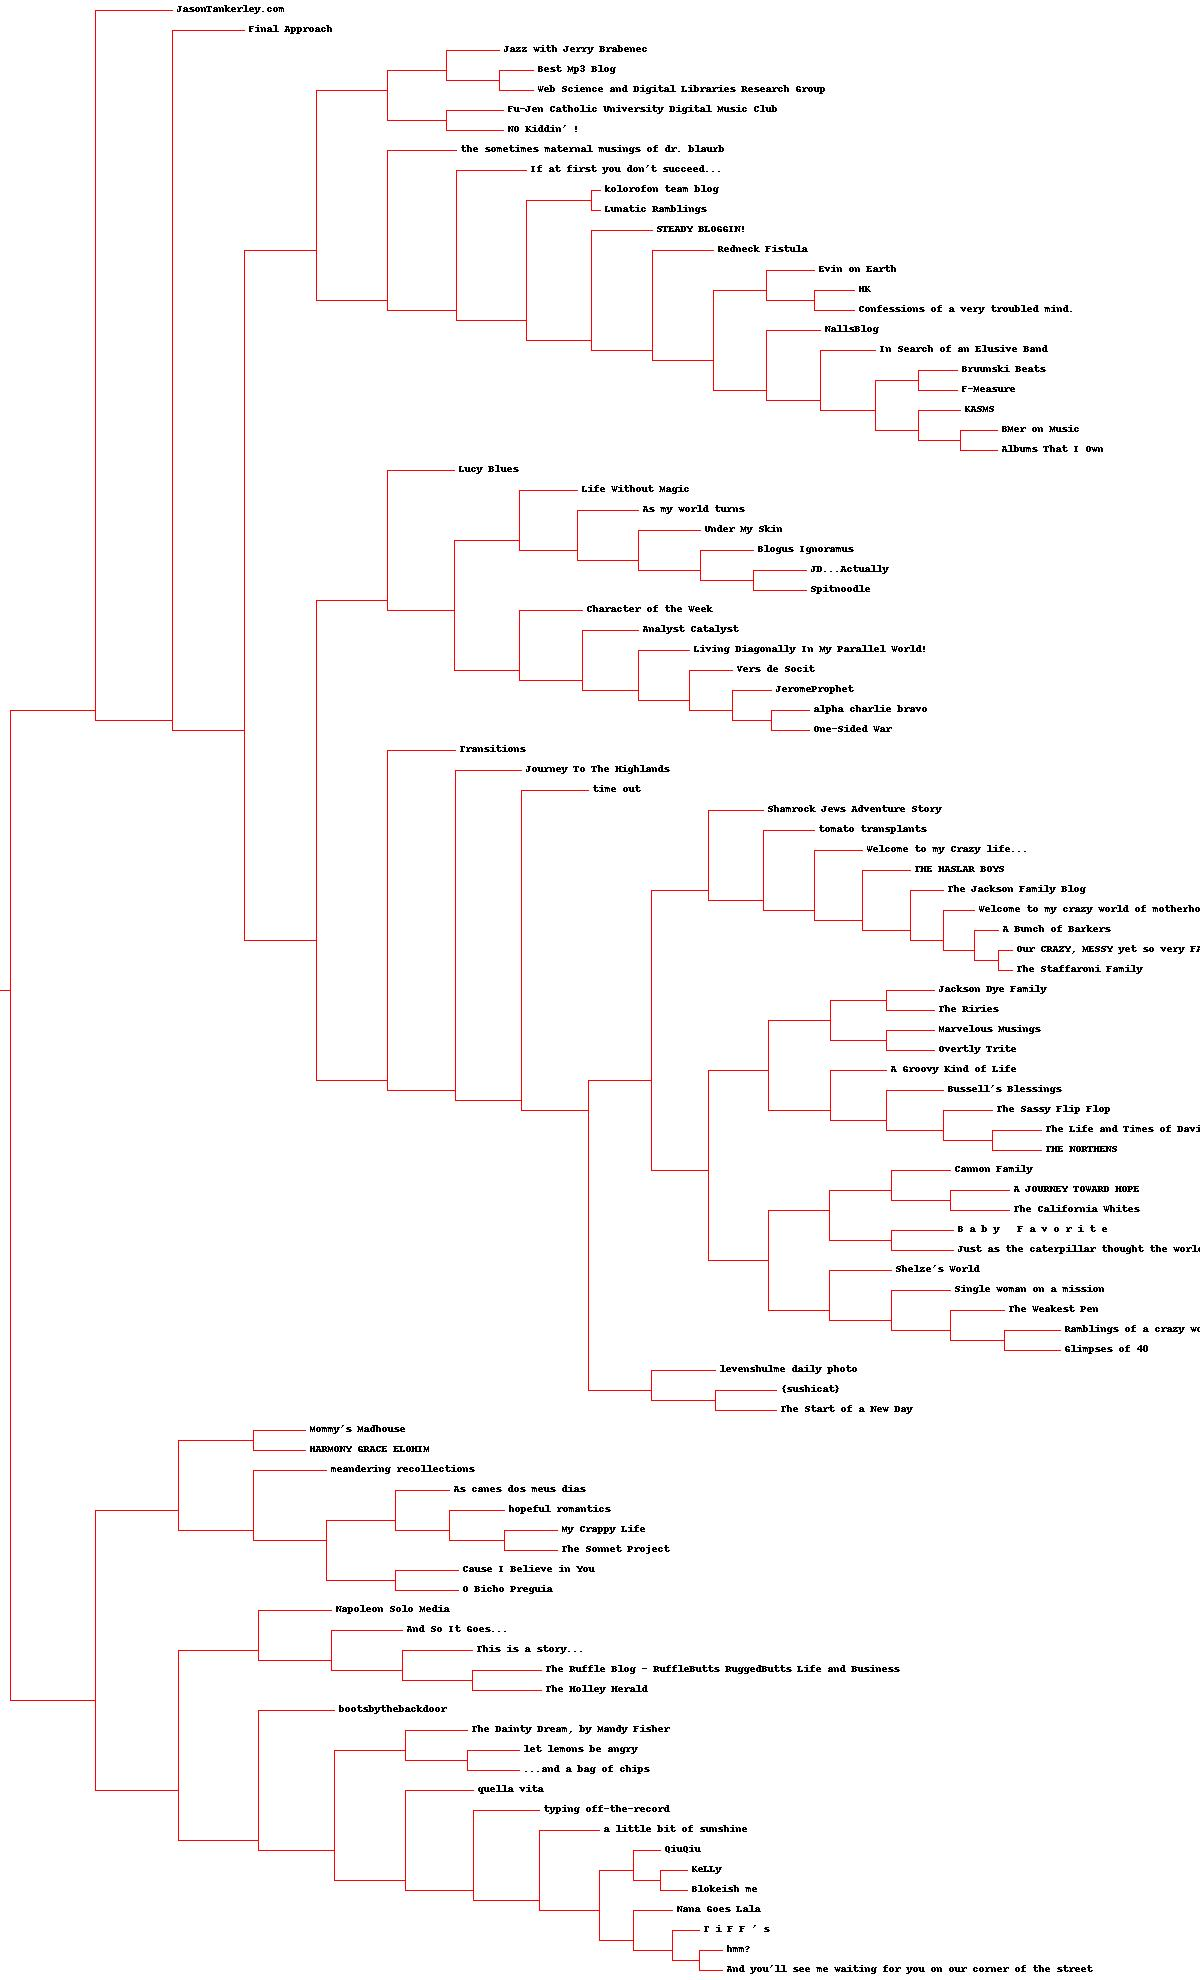
\includegraphics[width=\textwidth,height=.90\textheight]{../blogclust.jpg}}
\end{figure}

\end{enumerate}

\end{homeworkProblem}

%----------------------------------------------------------------------------------------
%   PROBLEM 3
%----------------------------------------------------------------------------------------
\begin{homeworkProblem}

Cluster the blogs using K-Means, using k=5,10,20. (see slide 18).
How many interations were required for each value of k?

\begin{verbatim}\end{verbatim}
\textbf{SOLUTION 3}\\


The solution for this problem is outlined by the following steps:
\begin{enumerate}

\item \textbf{Create clusters:} This was achieved due to Listing 8. Table 1. outlines the k-value/iteration tuples.
\lstinputlisting[breaklines=true, caption=Create Clusters]{createClustersSnippet.py}

\begin{verbatim}
    The file kMeansClusters.txt contains the clusterings/iteration count
    for k = 5, 10, 20
\end{verbatim}

\begin{table}[h]
    \caption{k-value vs Iteration Count} % title of Table
    \centering % used for centering table
    \begin{tabular}{c | c | c } % centered columns (4 columns)
    \hline\hline %inserts double horizontal lines
    ITEM & k-value & Iteration \\ [0.5ex] % inserts table 
    %heading
    \hline \hline% inserts single horizontal line
    1   &   5    &   5 \\ \hline
    2   &   10    &   7 \\ \hline
    3 & 20 & 5 \\ [1ex] 
    \hline %inserts single line
    \end{tabular}
    \label{table:nonlin} % is used to refer this table in the text
\end{table}

\end{enumerate}

\end{homeworkProblem}


%----------------------------------------------------------------------------------------
%   PROBLEM 4
%----------------------------------------------------------------------------------------
\begin{homeworkProblem}

Use MDS to create a JPEG of the blogs similar to slide 29.  
How many iterations were required?

\begin{verbatim}\end{verbatim}
\textbf{SOLUTION 4}\\


The solution for this problem is outlined by the following steps:
\begin{enumerate}

\item \textbf{Reduce dimension:} This was achieved due to Listing 9.
The iteration count was achieved by imposing a counter as long as the error continued to drop across iterations. Figure 3. Shows the resultant blog matrix in 2d.
\lstinputlisting[breaklines=true, caption=Create MDS]{createMDSSnippet.py}

\begin{figure}
    \caption{MDS Diagram, iterationCount = 226}
    \subfigure{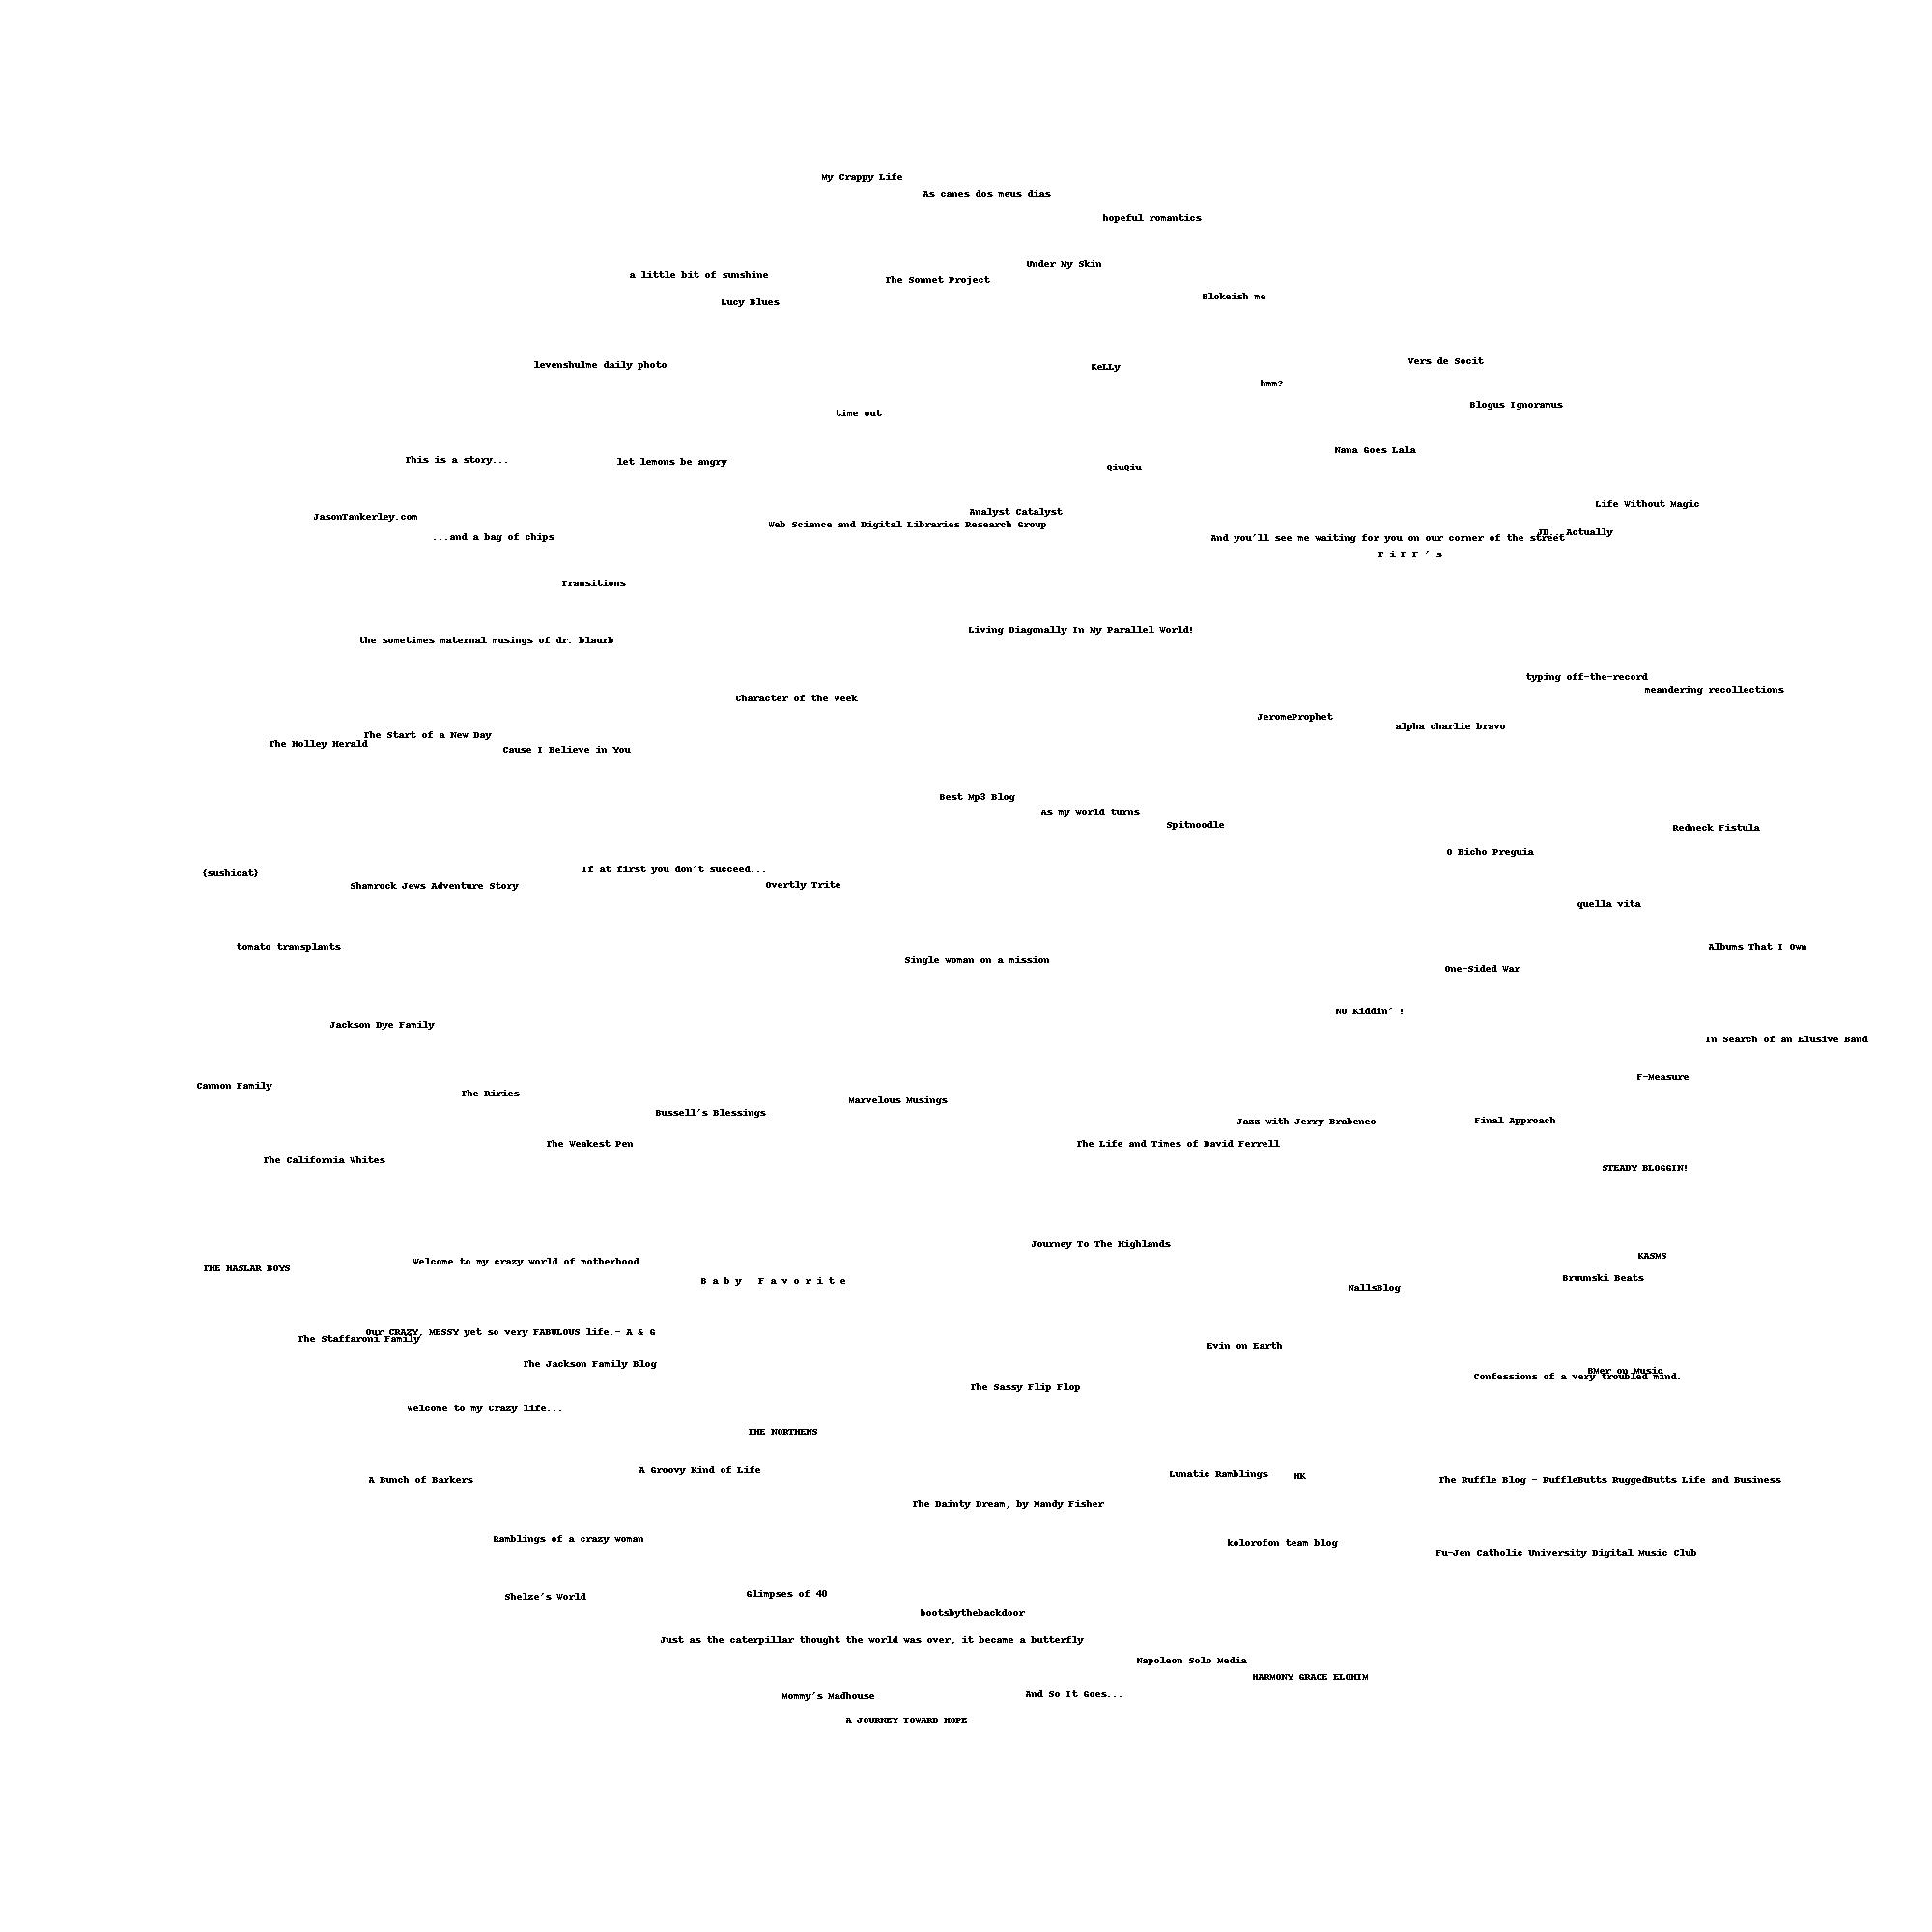
\includegraphics[width=\textwidth,height=.90\textheight]{../blogs2d.jpg}}
\end{figure}


\end{enumerate}

\end{homeworkProblem}

%----------------------------------------------------------------------------------------
%   PROBLEM 5
%----------------------------------------------------------------------------------------
\begin{homeworkProblem}

Re-run question 2, but this time with proper TFIDF calculations
instead of the hack discussed on slide 7 (p. 32).  Use the same 500
words, but this time replace their frequency count with TFIDF scores
as computed in assignment \#3.  Document the code, techniques,
methods, etc. used to generate these TFIDF values.  Upload the new
data file to github.\\

Compare and contrast the resulting dendrogram with the dendrogram
from question \#2.\\

Note: ideally you would not reuse the same 500 terms and instead
come up with TFIDF scores for all the terms and then choose the top
500 from that list, but I'm trying to limit the amount of work
necessary.

\begin{verbatim}\end{verbatim}
\textbf{SOLUTION 5}\\


The solution for this problem is outlined by the following steps:
\begin{enumerate}

\item \textbf{Calculate TFIDF values:} This was achieved by replacing the word count in generateFeedVector() with the TFIDF values as outlined by Listing 10. Given a word (w) in a file (f), Listing 10. computes the term frequency of w by dividing the word count of w by the length of f (total number of words). And the inverse document frequency is computed by dividing the corpus length by the total number of files which contain w. Thereafter, the term frequency-inverse document frequency is computed by multiplying the term frequency by the log of the inverse document frequency.

\lstinputlisting[breaklines=true, caption=Blog Matrix For TFIDF]{blogTFIDFVersionSnippet.py}

\item \textbf{Create dendogram:} Similar to the first dendogram, Figure 4. outlines the dendogram resulting from using TFIDF values instead of word counts.\\

\begin{figure}
    \caption{Blogs Dendogram (TFIDF Variant)}
    \subfigure{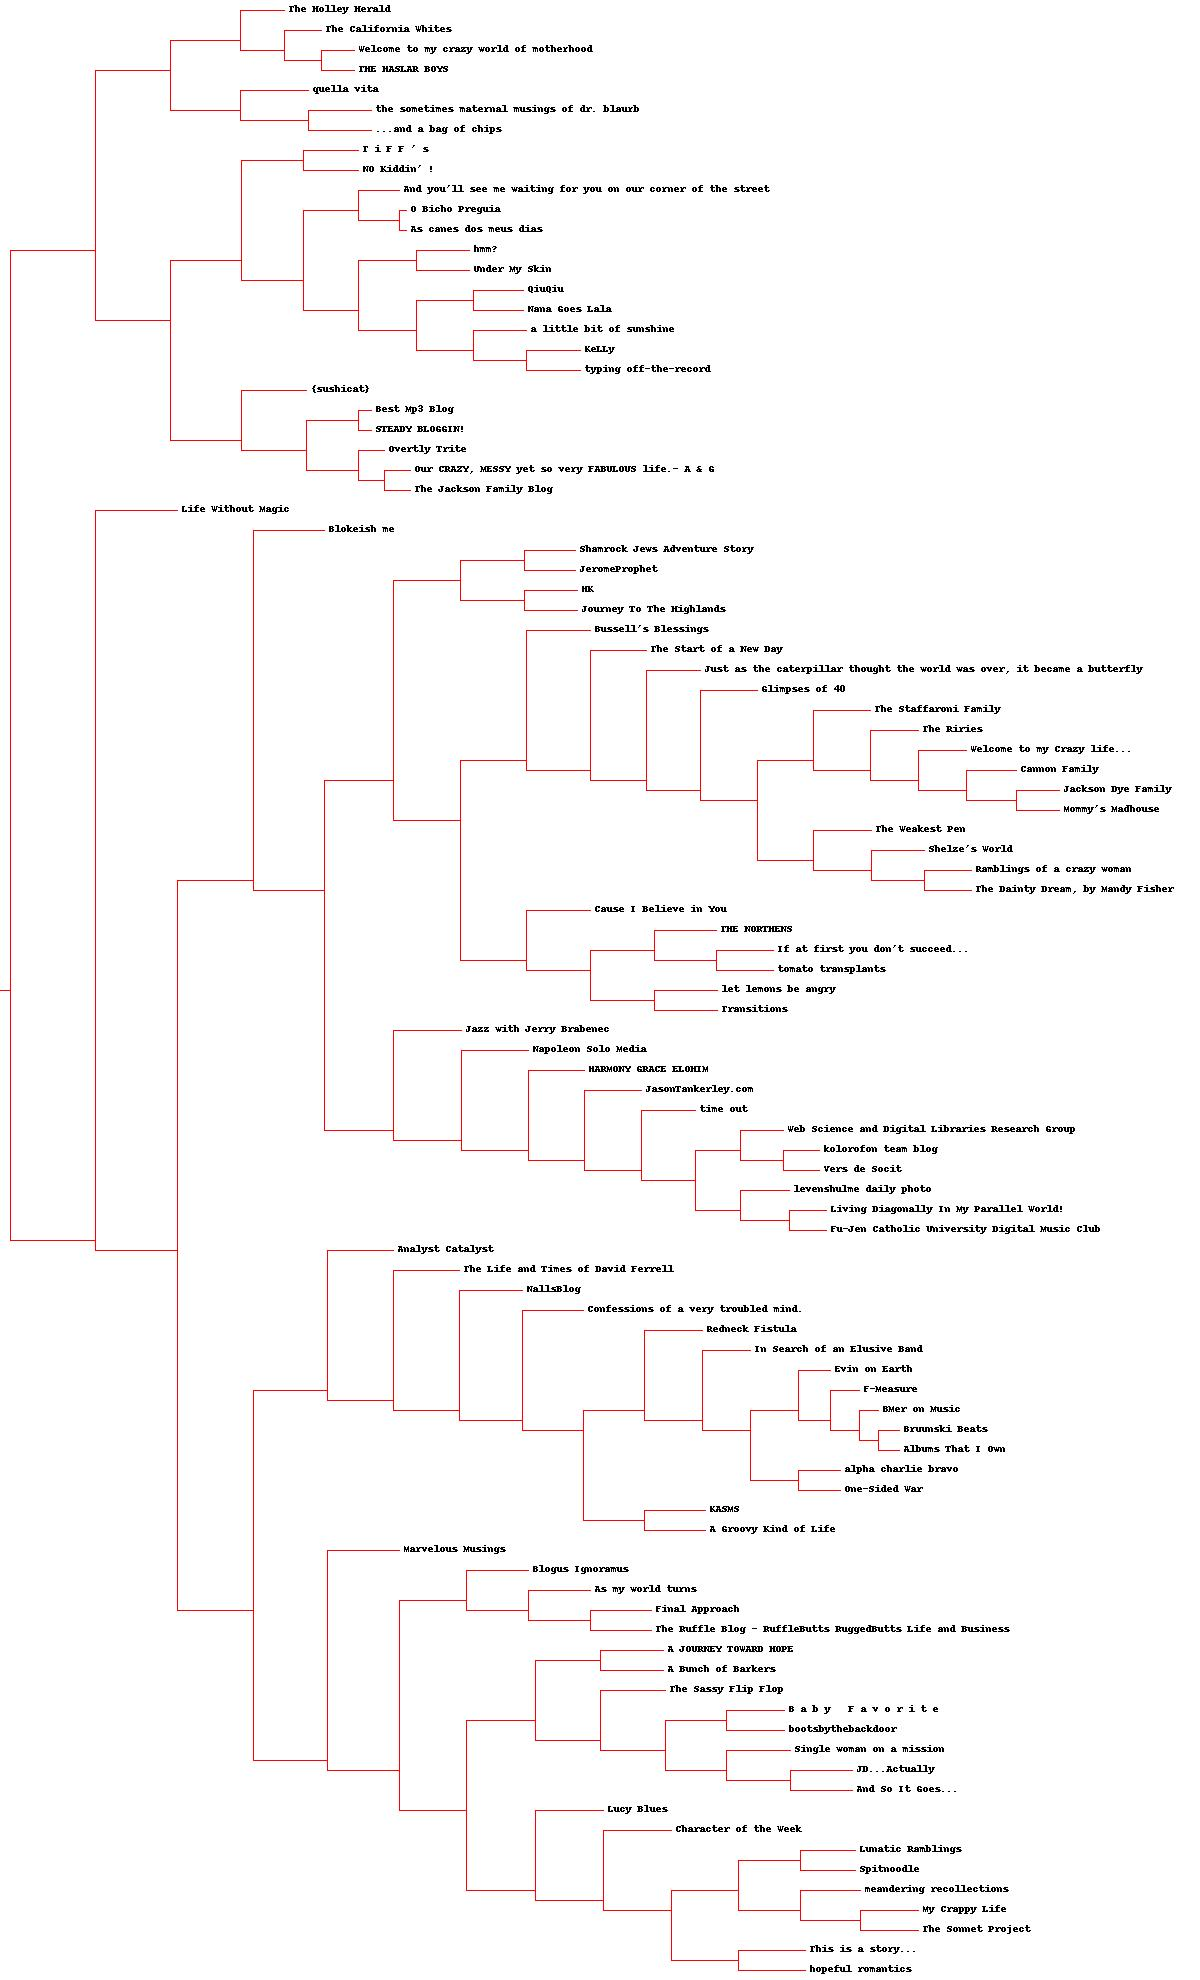
\includegraphics[width=\textwidth,height=.90\textheight]{../blogclustTFIDFVersion.jpg}}
\end{figure}


\textbf{Comparison/Contrast - (Figure 2 and Figure 4)}\\

The blogs dendogram due to TFIDF is more balanced compared to the blogs dendogram (word count) which is more skewed (unbalanced partitions). Also, the blogs dendogram (TFIDF) contains more clusters meaning TFIDF does a more fine-grained similarity comparison.\\

Although structurally the dendograms look dissimilar, semantically they are similar. Take the random cluster neigborhood of the F-measure blog as outlined in Figure 5, it can be seen that a couple of blogs are common within the neighborhood of F-measure.

\begin{figure}
    \caption{Similarity Of Dendograms (TFIDF (left) vs. Word Count(Right) ) Around F-measure Neighborhood}
    \subfigure{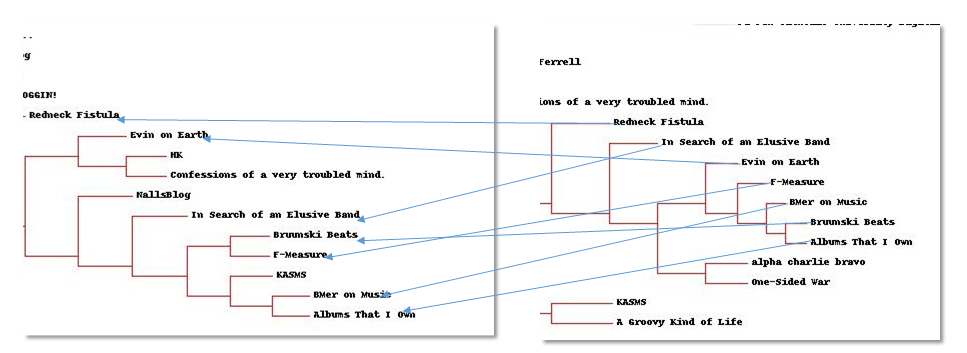
\includegraphics[width=\textwidth]{../fmNeighborhood.png}}
\end{figure}


\end{enumerate}

\end{homeworkProblem}

\begin{verbatim}


















\end{verbatim}

\bibliographystyle{plain}
\bibliography{A9bibFile}

%----------------------------------------------------------------------------------------

\end{document}